\section{Pruebas de hipótesis}
\begin{itemize}
    \item Inferencia estadística: dar conclusiones de la población (parámetros: $\mu, \sigma^2 , \sigma, p$) a partir de una muestra (estadísticos: $\bar{x}, s^2, s, \bar{p}$).
        \begin{itemize}
            \item $s$ $\longrightarrow$ $\sigma$
            \item $s^2$ $\longrightarrow$ $\sigma^2$   
            \item $\bar{p}$ $\longrightarrow$ $p$   
        \end{itemize}
\end{itemize}

\subsection{Inferencia estadística}
\begin{itemize}
    \item Intervalos de confianza 
    \item pruebas de hipótesis
\end{itemize}

\subsection{Pruebas de hipótesis}
\begin{figure}[H]
    \centering
    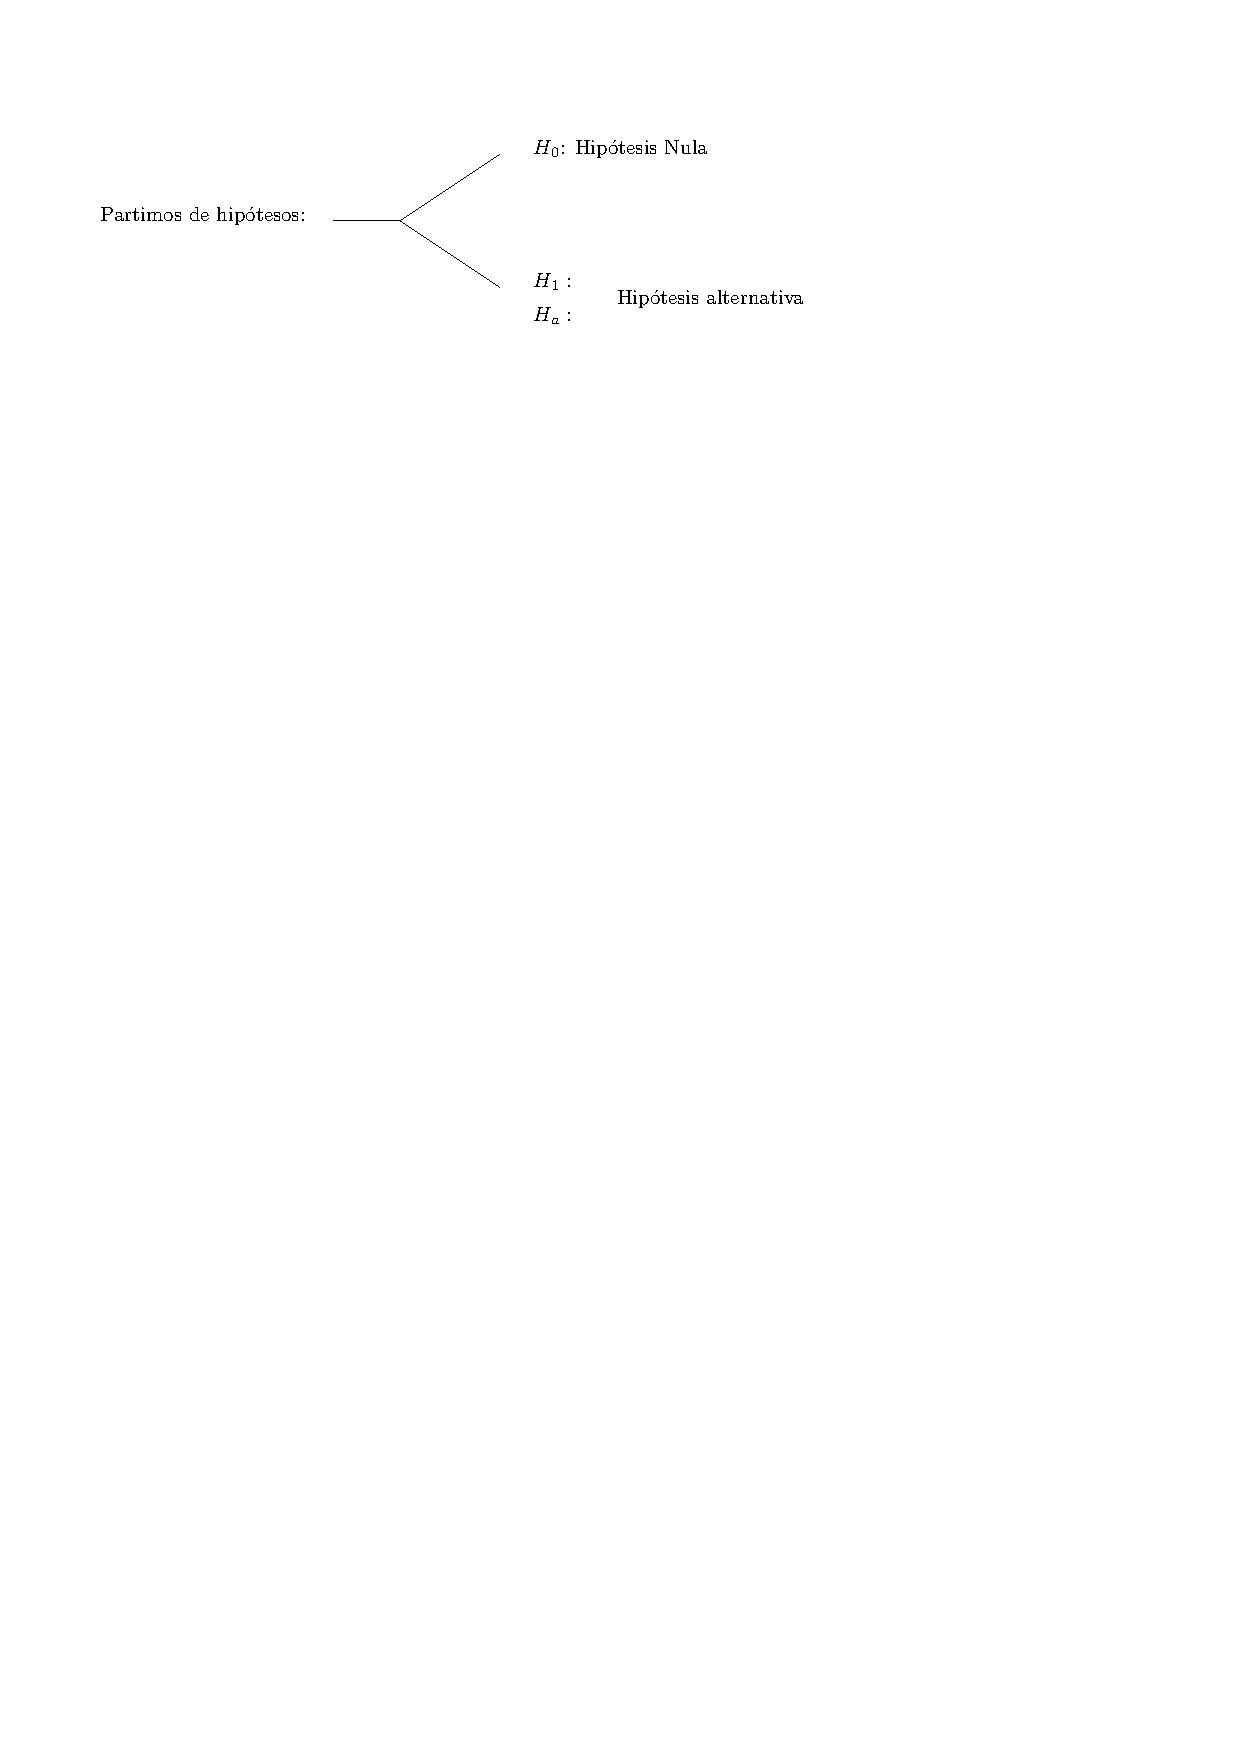
\includegraphics[width=14cm]{\figs/hipotesis} 
\end{figure}

\subsection{Ejemplo}
Una empresa azucarera tiene como producto líder, su presentación de 100 libras. Se sopecha que en promedio, dicho producto NO pesa 100 libras. 
\begin{enumerate}
    \item Parámetros de interés $\mu $.
    \item Hipótesis:
        \[
            \begin{array}{lrcc}
                H_0: & \mu = 100\qq    & \mu \leq 100 \qq & \mu \geq 100\qq \\
                H_a: & \mu \neq 100 \qq & \mu > 100 \qq & \mu < 100 \qq \\
            \end{array}
        \]
        \begin{itemize}
            \item La hipótesis nula siempre va a tener la igualdad.
            \item Este es un método alternativo a hacer lo del intervalo de confianza.
        \end{itemize}
        \begin{figure}[H]
            \centering
            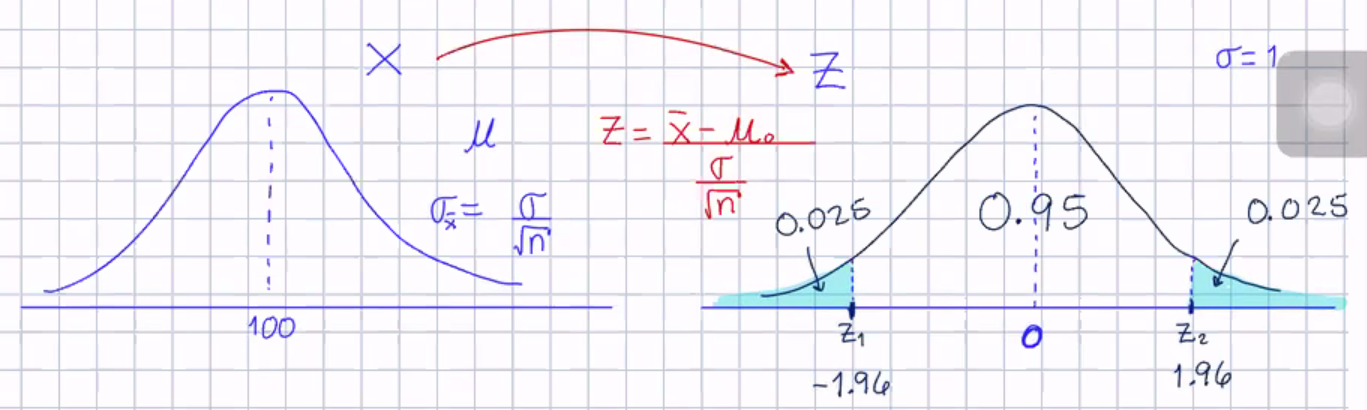
\includegraphics[width=14cm]{\figs/dist} 
        \end{figure}
    
    \item Asumimos como verdad lo siguiente:
        \begin{figure}[H]
            \centering
            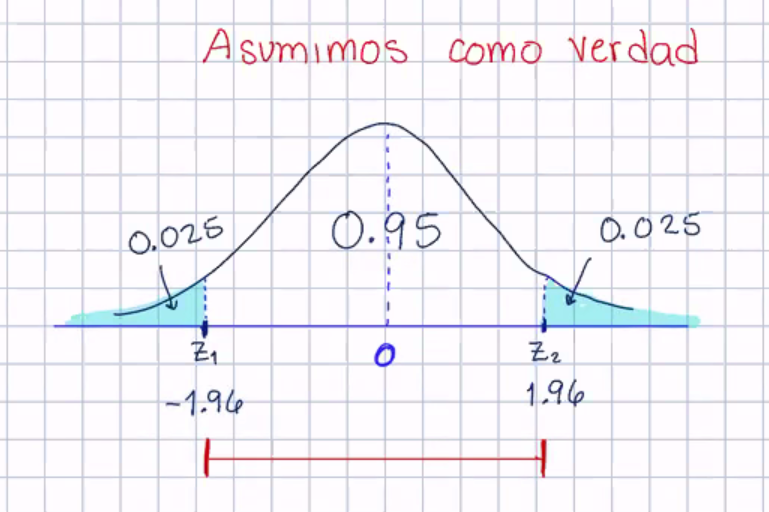
\includegraphics[width=14cm]{\figs/dist1} 
        \end{figure}
        \begin{itemize}
            \item Si la distribución fuera la correcta el 95\% de todas las medias muestrales estarían en este intervalo.
        \end{itemize}
    
    \item Si $\bar{x}$ cae en las colas (poco probable asumiendo que la distribución es verdadera).
        \begin{itemize}
            \item Por ende rechazamos $H_0$ 
        \end{itemize}
    
    \item Por ende la hipótesis nula no es verdadera.
\end{enumerate}



 
